%%%%%%%%%%%%%%%%%%%%%%%%%%%%%%%%%%%%%%%%%


\documentclass{beamer}

\mode<presentation> {


\usetheme{Madrid}




\usepackage{graphicx} 
\usepackage{booktabs} }

\title[Short title]{Introduction to AI /ML }

\author{Ujjwal (ee18btech11010) \\ Pranay (ee18btech11009)}
\institute[IITH] 
{
Indian Institute of Technology\\ 
\medskip
\textit{hyderabad}
}
\date{February 14, 2019}

\begin{document}

\begin{frame}
\titlepage 
\end{frame}

\begin{frame}
\frametitle{Question No. 22 (Geometric form)} 
22.  If an equilateral triangle ,having centroid at the origin , has a side along the line \\
           \[ x + y = 2,\]\\ then find the area of the triangle.
\end{frame}


%-----------------------------------------------------------------------------------
\begin{frame}
\frametitle{Question No. 22 (Matrix form)}
22. If an equilateral triangle , having centroid at the origin, has a side along the line 
\\
\quad \quad\quad\quad\quad \quad\quad\quad \quad\quad \begin{pmatrix}
1 & 1
\end{pmatrix}
\begin{pmatrix}
x \\ y
\end{pmatrix} = 2
\\
then find the area of the triangle .

\end{frame}

%------------------------------------------------

\begin{frame}
\frametitle{Solution}
Given the equation of the line along which the side of the equilateral triangle is,
\\ \[x + y = 2, \quad \quad \quad \quad \quad  . . . . . . . . .(1)\] \\ So, let  A = (2 & 0)  , B = (0 & 2 ) be two points on  x+y = 2 .\\
So, we have the direction vector of the line is ,\\
\quad \quad \quad \quad \quad \quad \quad \quad\begin{pmatrix}
2 & 0\\ 0 & 2 
\end{pmatrix}
\begin{pmatrix}
1 \\ -1 
\end{pmatrix}
=
2\begin{pmatrix}
1 \\ -1 

\end{pmatrix}
= d (A)\\
\quad Now, let Q(x & y) be the foot of the perpendicular\quad  from \quad  the  \quad origin  \quad   O (0 ,0) on the line    x+y = 2.
\end{frame}

%------------------------------------------------


.\\ .\\  So, we have the direction vector of OQ,
\\
\quad  \quad \quad \quad \quad  \quad \quad \quad OQ = d(B) = Q - O = 
\begin{pmatrix}
x \\y 
\end{pmatrix}\\
Since, the centroid and orthocenter of a equilateral triangle are same.\\ 
 we know that d(A) and d(B) are perpendicular .\\
  \quad \quad So, \\
   \quad \quad \quad \quad \quad \quad\implies d(A)^T d(B) = 0 \\ 
.   \\   \quad \quad \quad \quad \quad \quad \  \implies 2 
     \begin{pmatrix}
     x & y 
       \end{pmatrix}
       \begin{pmatrix}
       1 \\ -1
       \end{pmatrix}= 0\\ . \\
        \quad \quad
\ \quadend{ \quad   \quad\quad  \quad \quad \quad \quad\quad  x - y = 0 \quad \quad \quad \quad \quad \quad \quad \quad   . . . . . . . . . .(2)\\ 
Combining the equations (1)  and  (2), \\. \\
\quad \quad \quad \quad \quad \quad \quad \quad \quad \begin{pmatrix}
x \\ y
\end{pmatrix} 
\begin{pmatrix}
1 & 1 \\ 1 & -1 
\end{pmatrix} =
\begin{pmatrix}
2 \\ 0
\end{pmatrix} 

%------------------------------------------------

\begin{frame}
\frametitle{continuation . . .}

\quad \quad \quad \quad \quad  \implies Q = \begin{pmatrix}
x \\ y
\end{pmatrix} = 
\begin{pmatrix}
1 & 1 \\ 1 & -1 
\end{pmatrix} ^{-1}
\begin{pmatrix}
2 \\ 0
\end{pmatrix} = 
\begin{pmatrix}
1 \\ 1
\end{pmatrix}  
\\ . \\
Now we have ,\\ \quad\quad\quad lenght = OQ =  \sqrt{(1-0)^2 + (1-0)^2} = \sqrt{2}\\
Now, in an equilateral triangle with side 'a' and height 'h' ,\\
 \quad\quad\quad\quad\quad\quad \quad\quad\quad h = \sqrt{3}a/2\\ 
 We also know that the centroid divides the median in the ratio 2:1 \\
 \quad\quad\quad\quad\quad\quad\quad \implies CO : OQ  = 2 : 1
\end{frame}

%------------------------------------------------

\begin{frame}
\frametitle{}
So, \\  \quad\quad\quad\quad\quad\quad\quad  OQ = (1/3)h  =  a/2\sqrt{3}\\ . \\
 \quad\quad\quad\quad\quad\quad\quad \implies a = OQ(2\sqrt{3})  \\
 We know that the area of a equilateral triangle with side 'a' is,\\
  \quad\quad\quad\quad\quad\quad\quad A = \sqrt{3}{a}^2\4\\
   \quad\quad\quad\quad\quad\quad\quad \implies A = \sqrt{3} * 4* 3*(OQ)^2\\
      \quad\quad\quad\quad\quad\quad\quad \implies A =  3\sqrt{3}(OQ)^2\\
      Substituting the value of OQ \\
      \quad\quad\quad\quad\quad\quad\quad  A = 3\sqrt{3}(\sqrt{2})^2\\
      \quad\quad\quad\quad\quad\quad\quad \implies A = 6\sqrt{3} sq.units




\end{frame}

%------------------------------------------------

\begin{frame}
\frametitle{Plotting and computed values}
We can calculate the three vertices of a triangle using the equations for parametric co-ordinates and distance formula.\\
So, we have \\
\quad\quad\quad\quad\quad\quad\quad A=(2\sqrt{2}\cos(\pi/12) , -2\sqrt{2}\sin(\pi/12) )  \\
\quad\quad\quad\quad\quad\quad\quad B = (-2\sqrt{2}\sin(\pi/12) , 2\sqrt{2}\cos(\pi/12) , )\\
\quad\quad\quad\quad\quad\quad\quad C =(1- \sqrt{12}  , 1- \sqrt{12}) 
\end{frame}

%------------------------------------------------

\begin{frame}
\frametitle{Comptation} 
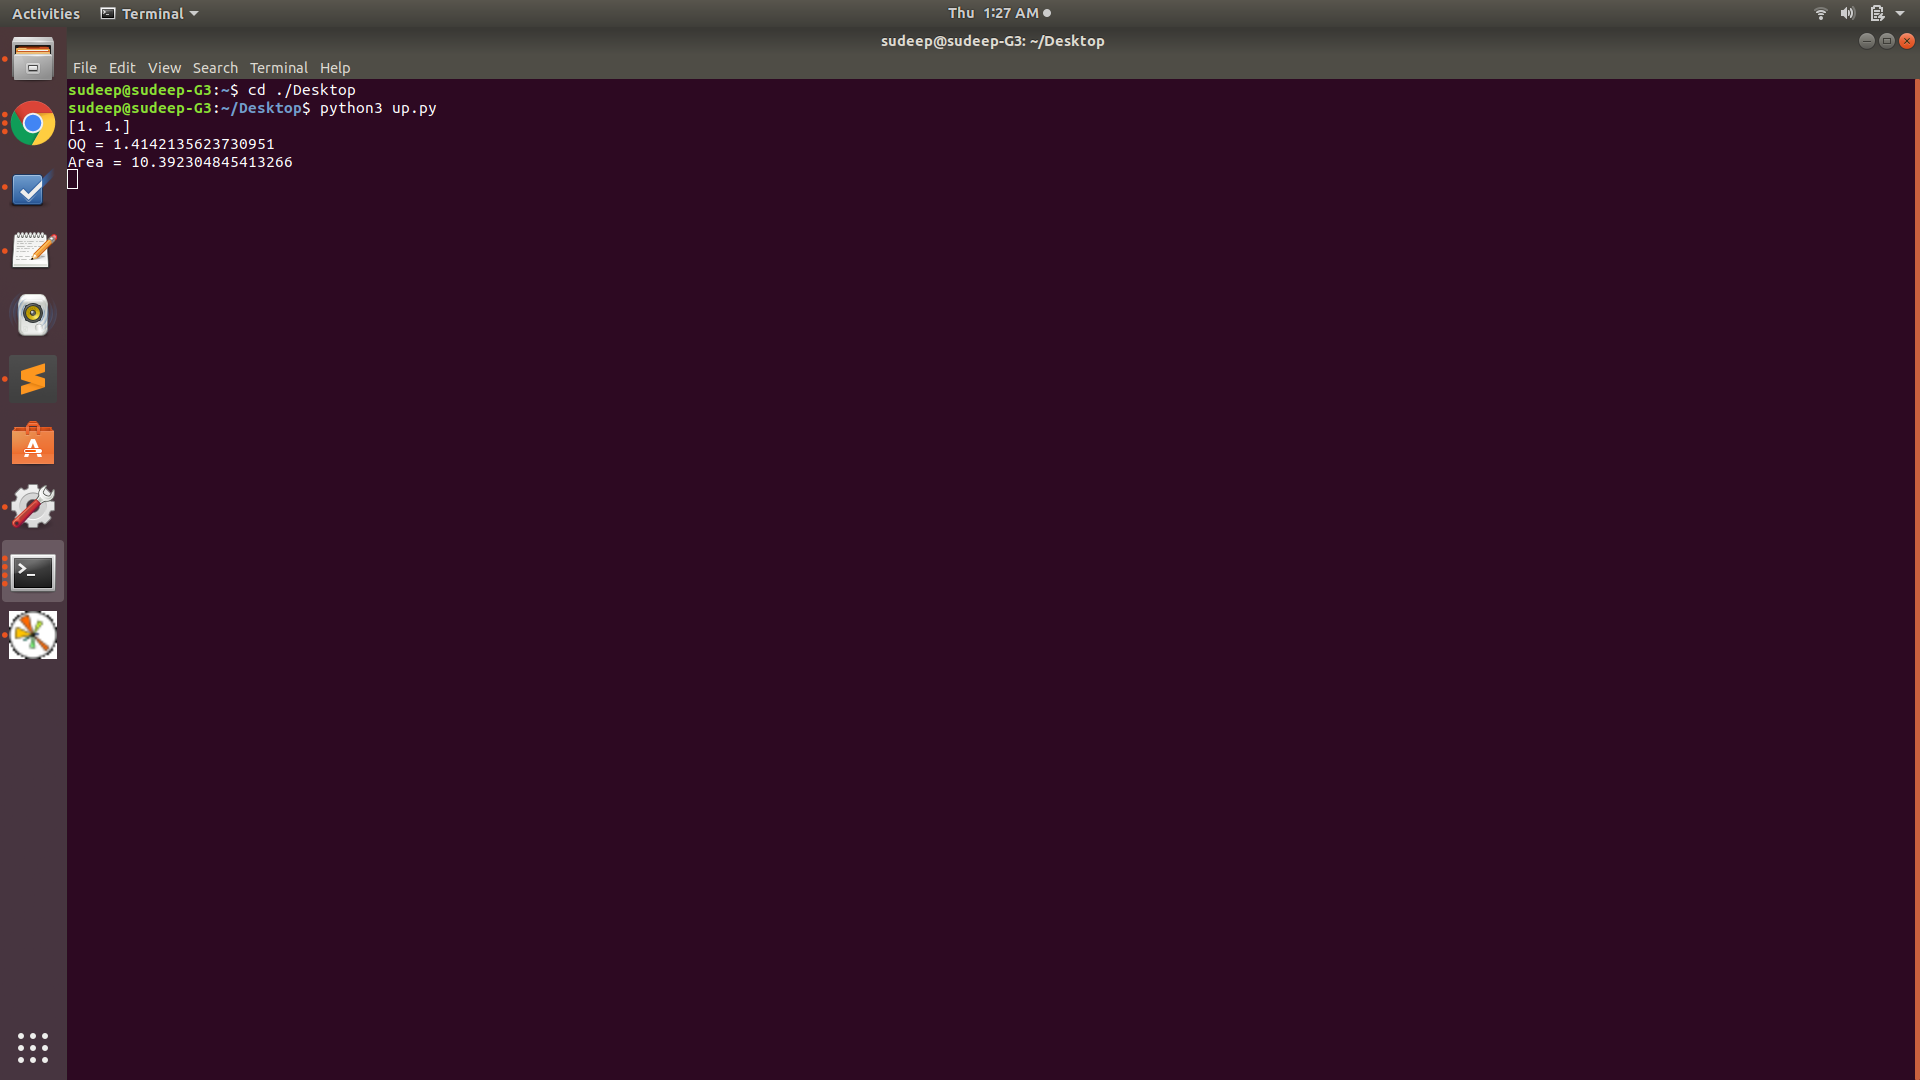
\includegraphics[scale = .8]{computation}
\end{frame}

%------------------------------------------------

\begin{frame}
\frametitle{graph}
\includegraphics[scale = .7]{up}
\end{frame}

%------------------------------------------------

\begin{frame}
\quad\quad\quad  \quad\quad\quad\quad\quad\quad \quad\quad\quad \quad\quad  THE END
\end{frame}
\end{document}